\documentclass[11pt,a4paper]{article}
\usepackage[T1]{fontenc}
\usepackage[margin=2.3cm]{geometry}
\usepackage{amsmath,amssymb}
\usepackage{graphicx}
\usepackage[dvipsnames]{xcolor}
\usepackage{enumitem}
\usepackage[colorlinks=true,linkcolor=blue,urlcolor=blue]{hyperref}
\setlength{\parskip}{0.6em}
\setlength{\parindent}{0pt}
\begin{document}

\begin{center}{\LARGE\bfseries openrecommend}\\[0.4em]{\large Build a recommender that suggests what you might like, in three sessions.}\\[0.2em]\small PAN IIT OSS explainer \textbullet{} higher secondary to advanced undergraduate (levels 4-6)\end{center}

\section*{Why this exists}
Every time an app says 'you might also like', it is making a guess from other people's ratings. This explainer shows the mathematics behind that guess, from an average gap on a table of 5 people to matrix factorisation, using only averages, dot products and a little algebra.

\section*{The end goal}
Build a recommender that suggests what you might like. The end goal is a working recommender that you built and tested honestly: it suggests what a user might like, you know how large its error is on ratings it has never seen, and you know where it fails (new users, overfitting, popularity bias).

\section*{How the three sessions build up}
\begin{enumerate}[nosep]
\item \textbf{Session 1: People who agree keep agreeing} (Level 1, conceptual interactive model, 60 min).
\item \textbf{Session 2: Measure similarity, predict, and test honestly} (Level 2, mathematical engineering model, 75 min).
\item \textbf{Session 3: Hidden tastes, cold start and shrinking variety} (Level 3, simulation and validation, 90 min).
\end{enumerate}

\section{Session 1: People who agree keep agreeing}

\subsection*{A. Real-world problem}
A video app has thousands of films and you have seen a handful. Which one should it show you next? It cannot read your mind, but it can look at other people who rated the same films as you and see what they liked next. Today you do this by hand on a table of 5 made-up people and 6 made-up films, then let Python repeat it. (This is education only: it is a teaching toy, not advice on what to watch or buy.)

\subsection*{B. Concept and theory}
A ratings table has one row per person and one column per film; each cell is a rating from 1 (hated it) to 5 (loved it), or empty if the person has not seen the film. To compare two people we look only at the films both have rated (the co-rated films), take the gap between their ratings on each film, ignore the sign, and average. A small average gap means similar taste. To guess a missing rating, find the k people with the smallest gap who have rated that film and average their ratings of it. The film with the highest guess is the recommendation.

\begin{itemize}[nosep]
\item r(a, f): rating of person a for film f (stars (1 to 5))
\item both: set of films rated by both persons (no unit)
\item gap(a, b): average absolute rating difference over the co-rated films (stars)
\item k: number of nearest people used for the guess (no unit)
\item guess(a, f): predicted rating of film f for person a (stars)
\end{itemize}

\begin{equation*}
\mathrm{gap}(a,b)=\frac{1}{|\mathrm{both}|}\sum_{f\in \mathrm{both}}\left|r(a,f)-r(b,f)\right|
\end{equation*}

\begin{equation*}
\mathrm{guess}(a,f)=\frac{1}{k}\sum_{b\in N_k(a,f)} r(b,f)
\end{equation*}

\begin{center}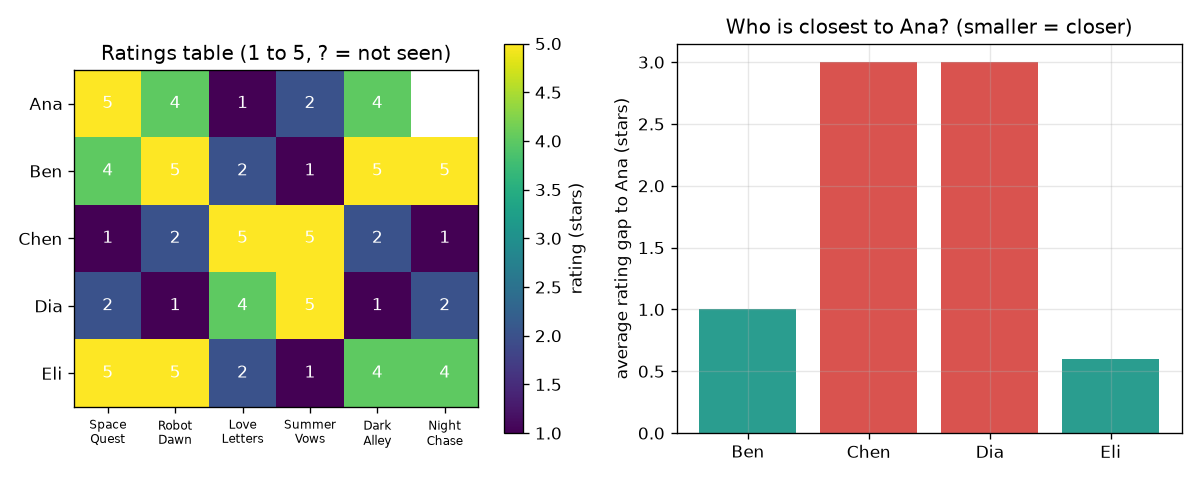
\includegraphics[width=0.85\linewidth]{figures/s01_ratings_and_gaps.png}\\\small Left: the 5 by 6 ratings table. Right: Eli is the closest person to Ana (gap 0.6 stars).\end{center}

\subsection*{E. Worked example}
Ana has not seen Night Chase. Use the table to guess her rating with 1 nearest person and with 2 nearest people.
\begin{enumerate}[nosep]
\item Compare Ana with Eli on the 5 films both rated: the gaps are 0, 1, 1, 1 and 0, so the average gap is 3 / 5 = 0.6 stars.
\item In the same way Ben has gap 5 / 5 = 1.0, and Chen and Dia each have gap 15 / 5 = 3.0.
\item The nearest person is Eli (0.6). Eli rated Night Chase 4, so the guess with k = 1 is 4 stars.
\item The two nearest people are Eli (0.6) and Ben (1.0). Ben rated Night Chase 5, so with k = 2 the guess is (4 + 5) / 2 = 4.5 stars.
\end{enumerate}
\textbf{Answer.} Guess 4 stars with one neighbour and 4.5 stars with two; Night Chase is the recommendation for Ana.

\subsection*{F. Questions}
\begin{enumerate}[nosep]
\item \textbf{Conceptual.} Why not simply recommend the film with the highest average rating to everybody? Name one situation where the neighbour method gives a better answer.
\item \textbf{Numerical.} Both Ben and Eli rated all 6 films: Ben gave 4, 5, 2, 1, 5, 5 and Eli gave 5, 5, 2, 1, 4, 4. Find the average rating gap between them and say whether they are similar. Give the unit.
\item \textbf{Graph and simulation interpretation.} In the bar chart of gaps to Ana, which two people are closest, and what does the guess become if we use all four people instead of the 2 nearest?
\item \textbf{Design and optimisation challenge.} Design: you may use k = 1, 2 or 4 neighbours to guess Ana's rating for Night Chase. Compare the three guesses and choose one. State the trade-off.
\end{enumerate}

\section{Session 2: Measure similarity, predict, and test honestly}

\subsection*{A. Real-world problem}
Session 1 compared 5 people by hand. A real service has thousands of users, each with a few dozen ratings, and you must turn 'similar taste' into a number, turn that number into a predicted rating, and then prove the predictions are any good. How do you test a recommender when you do not know the ratings people have not given yet? (Everything here is a synthetic teaching world; no real person is involved.)

\subsection*{B. Concept and theory}
For two users a and b take the items both rated and call the two lists of ratings x and y. Cosine similarity is the dot product of x and y divided by the product of their lengths. Pearson similarity is the same formula after subtracting each list's own mean, so it ignores whether a user rates everything high or low and only keeps the pattern. With plain 1 to 5 ratings every cosine is positive, so it separates users poorly. To predict, take the user's own mean rating and add the similarity-weighted average of what the k most similar users thought of the item, measured as how far each one's rating is above or below that user's own mean. Item-based prediction runs the same code on the transposed table, so items play the role of users. To evaluate, hide about 20\% of the known ratings and compare predictions with the truth: RMSE measures the typical error in stars, and the hit rate at N asks whether a liked hidden item appears in the top N list.

\begin{itemize}[nosep]
\item x, y: ratings of two users on their co-rated items (stars)
\item s(a, b): similarity of users a and b, between -1 and 1 (no unit)
\item mean\_u: average of the ratings user u has given (stars)
\item k: number of neighbours kept (no unit)
\item RMSE: root mean squared error on hidden ratings (stars)
\item hit rate@N: share of users with a liked hidden item in their top N (no unit)
\end{itemize}

\begin{equation*}
\cos(x,y)=\frac{x\cdot y}{\lVert x\rVert\,\lVert y\rVert}
\end{equation*}

\begin{equation*}
\mathrm{pearson}(x,y)=\frac{(x-\bar x)\cdot(y-\bar y)}{\lVert x-\bar x\rVert\,\lVert y-\bar y\rVert}
\end{equation*}

\begin{equation*}
\hat r(u,i)=\bar r_u+\frac{\sum_{v\in N_k}s(u,v)\,\big(r(v,i)-\bar r_v\big)}{\sum_{v\in N_k}\left|s(u,v)\right|}
\end{equation*}

\begin{equation*}
\mathrm{RMSE}=\sqrt{\frac{1}{n}\sum\big(\hat r-r\big)^2}
\end{equation*}

\begin{center}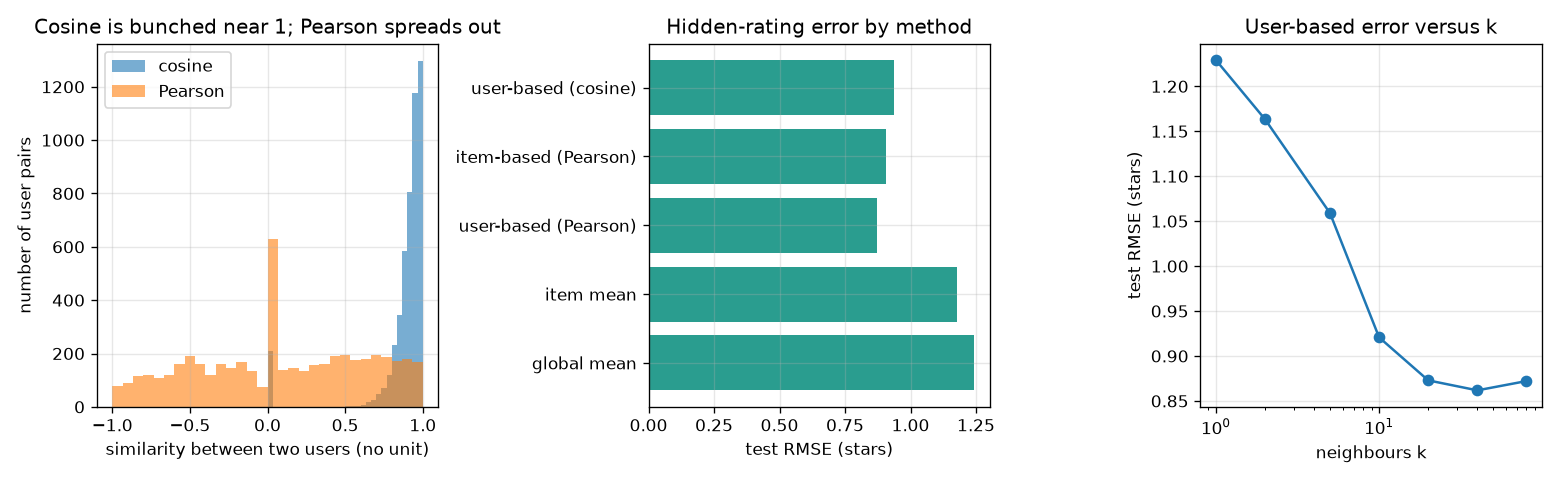
\includegraphics[width=0.85\linewidth]{figures/s02_similarity_and_error.png}\\\small Left: cosine versus Pearson over all user pairs. Middle: test RMSE by method. Right: user-based RMSE against the number of neighbours k.\end{center}

\subsection*{E. Worked example}
User A rated four items 5, 3, 4, 4 and has not rated item 5. User B rated them 3, 1, 2, 2 and gave item 5 a 3. Find cosine and Pearson between A and B on the 4 shared items, then predict A's rating for item 5 using B alone.
\begin{enumerate}[nosep]
\item Dot product: 5*3 + 3*1 + 4*2 + 4*2 = 15 + 3 + 8 + 8 = 34. Lengths: sqrt(25+9+16+16) = 8.124 and sqrt(9+1+4+4) = 4.243. Cosine = 34 / (8.124 * 4.243) = 0.986.
\item Pearson: A's mean is 4, so A - 4 = (1, -1, 0, 0). B's mean on the shared items is 2, so B - 2 = (1, -1, 0, 0). The two lists are identical, so Pearson = 1 exactly.
\item B's mean over all 5 of its ratings is (3 + 1 + 2 + 2 + 3) / 5 = 2.2, so B's surprise on item 5 is 3 - 2.2 = 0.8 stars.
\item With one neighbour of similarity 1 the weighted average of surprises is 0.8, so the prediction is A's own mean plus 0.8 = 4 + 0.8 = 4.8 stars.
\end{enumerate}
\textbf{Answer.} Cosine 0.986, Pearson 1.0, and the predicted rating of A for item 5 is 4.8 stars.

\subsection*{F. Questions}
\begin{enumerate}[nosep]
\item \textbf{Conceptual.} Why does Pearson similarity separate users better than cosine when all ratings are between 1 and 5? What does a negative Pearson mean?
\item \textbf{Numerical.} Two users share 3 items. User x rated them 5, 3, 1 and user y rated them 4, 4, 1. Compute the cosine and the Pearson similarity (no unit).
\item \textbf{Graph and simulation interpretation.} In the right panel, the error falls from 1.229 at k = 1. Roughly where is the best k, and why does the error rise again for very large k?
\item \textbf{Design and optimisation challenge.} Design: the checkpoint reports hit rate at 5 of 0.271 for random, 0.747 for popularity, 0.621 for user-based and 0.678 for item-based, but the RMSE of user-based is much better than popularity-like baselines. Which method would you ship for a 'top 5 picks' row, and what would you change in the test before trusting the answer?
\end{enumerate}

\section{Session 3: Hidden tastes, cold start and shrinking variety}

\subsection*{A. Real-world problem}
Neighbour methods compare raw pairs of users. A stronger idea is to assume every user and every item can be described by a few hidden numbers (taste factors) and to learn them so that 'user factors times item factors' reproduces the known ratings. Then the awkward questions: how many factors is too many, what do you show a brand-new user who has rated nothing, and what happens to the variety of what is shown when the system leans on popularity? (Education only: real systems must also respect people's privacy and fairness, and everything here is synthetic.)

\subsection*{B. Concept and theory}
Model: rating(u, i) is approximately mu + p\_u . q\_i, where mu is the average training rating and p\_u, q\_i are vectors of k hidden numbers for user u and item i. We minimise the squared error on the known training cells plus lambda times the squared lengths of all vectors; lambda (regularisation) punishes large vectors. If the item vectors are frozen, the best p\_u is a ridge regression with a closed form that uses only the items u has rated; likewise for the q\_i when the user vectors are frozen. Alternating the two solves is alternating least squares (ALS) and each half step can only lower the objective. The training error always falls as k grows, so we choose k and lambda on a separate validation set and quote the error once on a test set. If test ratings leak into training, the reported test error is fake. A new user has no ratings, so p\_u cannot be learned: we fall back to popularity, and after m ratings we fold in by solving the ridge problem for p\_u with the item vectors frozen. Diversity of a set of lists is measured by coverage (distinct items shown divided by catalogue size) and by the share of slots filled by the 10 most-rated items.

\begin{itemize}[nosep]
\item mu: average training rating (stars)
\item p\_u, q\_i: hidden taste vectors of user u and item i, k numbers each (no unit)
\item k: rank: number of hidden factors (no unit)
\item lambda: regularisation strength (no unit)
\item RMSE: root mean squared error (stars)
\item precision at 3: share of the 3 recommended items that the user likes (rating 4 or 5) (no unit)
\item coverage: distinct recommended items divided by catalogue size (no unit)
\end{itemize}

\begin{equation*}
\hat r(u,i)=\mu+p_u\cdot q_i
\end{equation*}

\begin{equation*}
J=\sum_{(u,i)\in\mathrm{train}}\big(r(u,i)-\mu-p_u\cdot q_i\big)^2+\lambda\Big(\sum_u\lVert p_u\rVert^2+\sum_i\lVert q_i\rVert^2\Big)
\end{equation*}

\begin{equation*}
p_u=\big(Q_u^{\mathsf T}Q_u+\lambda I\big)^{-1}Q_u^{\mathsf T}\,(r_u-\mu)
\end{equation*}

\begin{equation*}
\mathrm{coverage}=\frac{\#\{\text{distinct items in all lists}\}}{\#\{\text{items}\}}
\end{equation*}

\begin{center}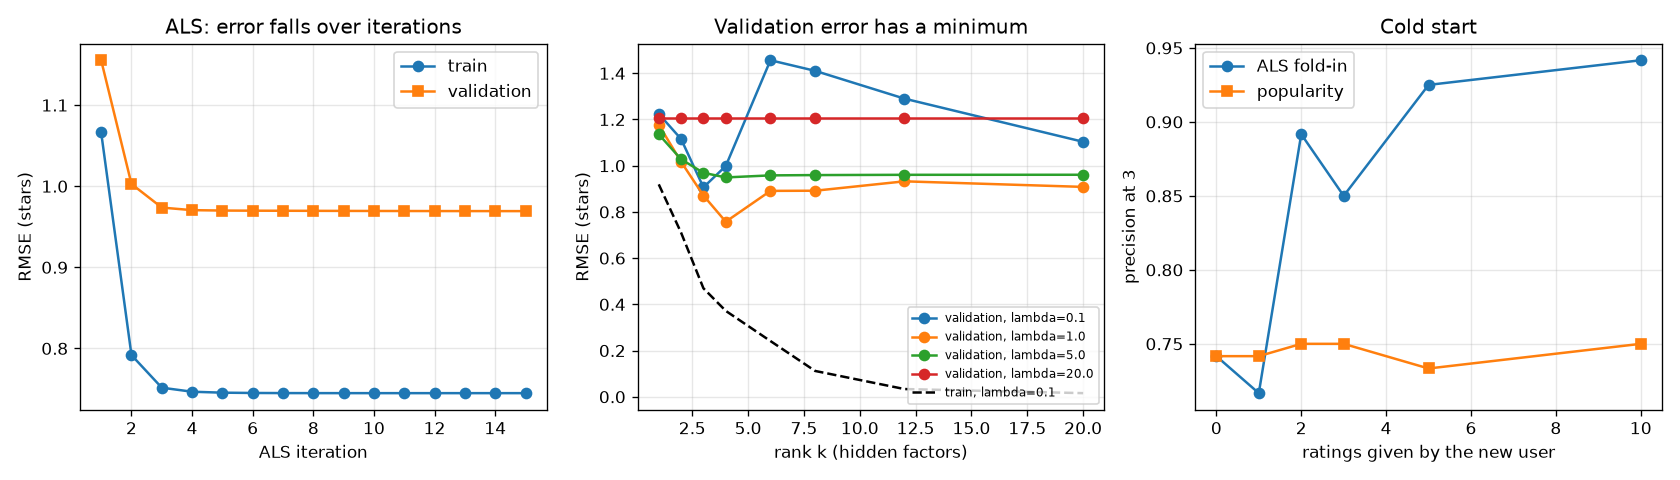
\includegraphics[width=0.85\linewidth]{figures/s03_als_validation_coldstart.png}\\\small Left: ALS error against iteration. Middle: validation error against rank k for four values of lambda, with the training error dashed. Right: cold-start precision at 3 against the number of ratings given.\end{center}

\subsection*{E. Worked example}
One ridge step by hand. Two items have one-number vectors q = 1 and q = 2. A user (with mu = 3) rated them 4 and 5, so the centred ratings are 1 and 2. Find the user's vector p for lambda = 1 and for lambda = 0, and the predicted rating for an item with q = 2.
\begin{enumerate}[nosep]
\item For one hidden factor, p = (sum of q * centred rating) / (sum of q squared + lambda).
\item Numerator: 1*1 + 2*2 = 5. Sum of q squared: 1 + 4 = 5.
\item With lambda = 1: p = 5 / (5 + 1) = 0.8333. With lambda = 0: p = 5 / 5 = 1, an exact fit (1*1 = 1 and 1*2 = 2).
\item Prediction for an item with q = 2: with lambda = 1 it is 3 + 0.8333*2 = 4.667; with lambda = 0 it is 3 + 1*2 = 5.
\end{enumerate}
\textbf{Answer.} p = 0.8333 (lambda = 1) against p = 1 (lambda = 0); regularisation shrinks the vector and the prediction from 5 to 4.667 stars.

\subsection*{F. Questions}
\begin{enumerate}[nosep]
\item \textbf{Conceptual.} Why can the training error go to zero while the model gets worse on new ratings? What is the role of lambda?
\item \textbf{Numerical.} Redo the worked example with the user's ratings 3 and 5 (centred ratings 0 and 2, mu = 3). Find p for lambda = 1 and lambda = 0 and the predicted rating for q = 2.
\item \textbf{Graph and simulation interpretation.} In the grid of validation errors, where is the minimum, and what happens in the column lambda = 20 for every k?
\item \textbf{Design and optimisation challenge.} Design: the onboarding screen of a new app can ask a new user for m ratings (0, 1, 2, 3, 5 or 10). Using precision at 3 for ALS fold-in (0.74, 0.72, 0.89, 0.85, 0.93, 0.94) and for popularity (0.74, 0.74, 0.75, 0.75, 0.73, 0.75), choose m and justify it. What would you do before the user has rated anything?
\end{enumerate}

\section{Real-world mini-project}
\textbf{Recommend 3 items for a new user and beat the popularity baseline.} A streaming app has 40 brand-new users. For each user, the app asks for m ratings of random items and then recommends 3 unseen items. Use \texttt{build\_world}, \texttt{als} (with k = 4 and lambda = 1), \texttt{cold\_start\_curve} and \texttt{popularity\_order} from Session 3. For m = 0, 1, 2, 3, 5 and 10 compute precision at 3 (the share of the 3 recommended items the user likes) for ALS fold-in and for the popularity baseline, then find the smallest m for which ALS beats popularity by at least 0.10.

\section{The path ahead}
\begin{enumerate}[nosep]
\item \textbf{Session 4: Add bias terms.} ALS where the model is mu plus a user bias plus an item bias plus the factor match, each bias solved in the same alternating loop.
\item \textbf{Session 5: A smarter cold start.} A recommender for new users that blends fold-in scores with item average ratings.
\item \textbf{Session 6: Variety-aware ranking.} A re-ranker that penalises items that have already been recommended to many users.
\item \textbf{Session 7: Closed-loop simulation.} A simulation of 8 rounds where every user is shown 5 unseen items, rates them with the true rating, and the model is refit.
\end{enumerate}

\section{Answers and hints}

\subsection*{Session 1}
\begin{enumerate}[nosep]
\item \textbf{Conceptual.} Hint: Think about two people with opposite tastes in the table. Solution: A global average treats Ana and Chen the same, even though their ratings disagree on every film. The neighbour method only listens to people who agree with Ana, so for a taste group that is a minority it recommends what that group likes (space films) rather than what the majority likes. Its weakness: it needs shared films to compare people, and it may be wrong when few people have rated the film.
\item \textbf{Numerical.} Hint: Take the absolute difference on each of the 6 films, add, divide by 6. Solution: The gaps are 1, 0, 0, 0, 1, 1, which add to 3; 3 / 6 = 0.5 stars. A gap of half a star on a 5-star scale means very similar taste. Sanity check: the gap can never be larger than 4 stars (1 against 5) and is 0 only for identical ratings.
\item \textbf{Graph and simulation interpretation.} Hint: Read the two smallest bars, then average everybody's rating of Night Chase (Ben 5, Chen 1, Dia 2, Eli 4). Solution: Eli (0.6) and Ben (1.0) are closest. Using all four people gives (5 + 1 + 2 + 4) / 4 = 3.0 stars: the two people who disagree with Ana pull the guess down from 4.5 to 3.0. This is why we use only the nearest people.
\item \textbf{Design and optimisation challenge.} Hint: Compute the guess for each k with \texttt{predict(RATINGS, 0, 5, k)} and compare with what Session 1 found by hand. Solution: k = 1 gives 4.0, k = 2 gives 4.5 and k = 4 gives 3.0. With k = 1 the guess rests on a single person, so one unusual rating can mislead; with k = 4 everybody counts, including people who disagree with Ana, so the guess ignores her taste. In a table this small k = 2 is a sensible compromise: two people who agree with her. With a bigger table a larger k averages out noise as long as the neighbours really are similar.
\end{enumerate}

\subsection*{Session 2}
\begin{enumerate}[nosep]
\item \textbf{Conceptual.} Hint: Cosine of two lists of positive numbers can never be below 0. What does subtracting the mean remove? Solution: With only positive ratings the dot product x . y is always positive, so cosine is always above 0 and mostly close to 1 (the checkpoint confirms no cosine is negative). Subtracting each list's own mean removes 'this user rates everything high' and keeps only the up-and-down pattern, so Pearson can be negative. A negative Pearson means the two users tend to disagree: when one rates an item above their own average, the other rates it below theirs.
\item \textbf{Numerical.} Hint: Cosine: dot product over product of lengths. Pearson: first subtract the mean (3 for both) from each list. Solution: Cosine: dot = 20 + 12 + 1 = 33; lengths sqrt(35) = 5.916 and sqrt(33) = 5.745; cosine = 33 / 33.99 = 0.971. Pearson: x - 3 = (2, 0, -2), y - 3 = (1, 1, -2); dot = 2 + 0 + 4 = 6; lengths 2.828 and 2.449; Pearson = 6 / 6.928 = 0.866. Both are below 1, and Pearson is the more demanding of the two.
\item \textbf{Graph and simulation interpretation.} Hint: Compare the values at k = 20, 40 and 80 (0.873, 0.862, 0.872). Solution: The lowest value is 0.862 stars at k = 40; at k = 20 it is 0.873 and at k = 80 it is 0.872, so the curve is flat near the minimum. With k = 1 a single noisy neighbour decides; as k grows noise averages out. For very large k users who are not really similar are included and pull every prediction towards the crowd, so the error stops improving and creeps up.
\item \textbf{Design and optimisation challenge.} Hint: Remember which cells are hidden: only ratings that people actually gave, and popular items get more of them. Solution: On this test popularity wins the top-5 task (0.747 against 0.621 and 0.678), although the neighbour methods predict individual ratings much better (RMSE 0.873 and 0.906 against 1.179 for the item mean). The hidden test cells come from the same exposure-biased process as the training cells, so popular items dominate them and reward a popularity ranking. Before shipping I would test on ratings collected with random exposure, measure more than hit rate (for example variety and novelty), and probably combine popularity with personal scores. Trade-off: the safest pick is not the most personal one.
\end{enumerate}

\subsection*{Session 3}
\begin{enumerate}[nosep]
\item \textbf{Conceptual.} Hint: With k = 20 factors per user and only a handful of ratings per user, how many numbers are being fitted per rating? Solution: With many factors the model has enough freedom to memorise every training rating, noise included, so the training error falls (to 0.016 stars at k = 20, lambda = 0.1) while the validation error is 1.103 stars. It has learned the noise, not the tastes. Lambda punishes long vectors, so a larger lambda limits the memorising: at k = 20 raising lambda from 0.1 to 1 lowers the validation error from 1.103 to 0.908.
\item \textbf{Numerical.} Hint: p = (sum of q * centred rating) / (sum of q squared + lambda); the numerator is 1*0 + 2*2. Solution: Numerator 4, sum of q squared 5. Lambda = 0: p = 4/5 = 0.8 and the prediction for q = 2 is 3 + 0.8*2 = 4.6 stars. Lambda = 1: p = 4/6 = 0.667 and the prediction is 3 + 0.667*2 = 4.333 stars. The regularised fit is pulled towards 0, towards the plain average rating of 3.
\item \textbf{Graph and simulation interpretation.} Hint: Read the smallest number in the grid; look at the lambda = 20 row. Solution: The minimum is 0.758 stars at k = 4, lambda = 1. For lambda = 20 the validation error is 1.208 for every k: the penalty is so heavy that all vectors collapse to zero and the model just predicts the average rating mu. That is underfitting, the opposite failure to overfitting.
\item \textbf{Design and optimisation challenge.} Hint: Where does the ALS curve cross the popularity curve, and where does it flatten? Solution: With 0 ratings ALS has nothing to learn from and equals popularity (0.74), so show popular items. With 1 rating ALS is not yet better (0.72 against 0.74). From 2 ratings on it beats popularity clearly (0.89 against 0.75), and at 5 ratings it reaches 0.93; the step from 5 to 10 adds only 0.01. Asking for 5 ratings is a sensible trade-off between effort for the user and accuracy. Caveat: only 40 new users were simulated, so the curve is not smooth (3 ratings scores below 2); treat differences of a few hundredths as noise.
\end{enumerate}

\section{How to join}
Read \texttt{CONTRIBUTING.md} in the repository, then pick an issue labelled \texttt{good first issue}. Repository: \url{https://github.com/KrunalPanchal1995/openrecommend}

\end{document}
